% Options for packages loaded elsewhere
\PassOptionsToPackage{unicode}{hyperref}
\PassOptionsToPackage{hyphens}{url}
%
\documentclass[
]{article}
\usepackage{amsmath,amssymb}
\usepackage{lmodern}
\usepackage{iftex}
\ifPDFTeX
  \usepackage[T1]{fontenc}
  \usepackage[utf8]{inputenc}
  \usepackage{textcomp} % provide euro and other symbols
\else % if luatex or xetex
  \usepackage{unicode-math}
  \defaultfontfeatures{Scale=MatchLowercase}
  \defaultfontfeatures[\rmfamily]{Ligatures=TeX,Scale=1}
\fi
% Use upquote if available, for straight quotes in verbatim environments
\IfFileExists{upquote.sty}{\usepackage{upquote}}{}
\IfFileExists{microtype.sty}{% use microtype if available
  \usepackage[]{microtype}
  \UseMicrotypeSet[protrusion]{basicmath} % disable protrusion for tt fonts
}{}
\makeatletter
\@ifundefined{KOMAClassName}{% if non-KOMA class
  \IfFileExists{parskip.sty}{%
    \usepackage{parskip}
  }{% else
    \setlength{\parindent}{0pt}
    \setlength{\parskip}{6pt plus 2pt minus 1pt}}
}{% if KOMA class
  \KOMAoptions{parskip=half}}
\makeatother
\usepackage{xcolor}
\IfFileExists{xurl.sty}{\usepackage{xurl}}{} % add URL line breaks if available
\IfFileExists{bookmark.sty}{\usepackage{bookmark}}{\usepackage{hyperref}}
\hypersetup{
  pdftitle={Supplementary materials for `Unusually warm winter seasons may compromise the performance of current phenology models - Predicting bloom dates in young apple trees with PhenoFlex'},
  pdfauthor={Eduardo Fernandeza,b, Katja Schiffersa, Carsten Urbachc and Eike Luedelinga},
  hidelinks,
  pdfcreator={LaTeX via pandoc}}
\urlstyle{same} % disable monospaced font for URLs
\usepackage[margin=1.5cm]{geometry}
\usepackage{color}
\usepackage{fancyvrb}
\newcommand{\VerbBar}{|}
\newcommand{\VERB}{\Verb[commandchars=\\\{\}]}
\DefineVerbatimEnvironment{Highlighting}{Verbatim}{commandchars=\\\{\}}
% Add ',fontsize=\small' for more characters per line
\usepackage{framed}
\definecolor{shadecolor}{RGB}{248,248,248}
\newenvironment{Shaded}{\begin{snugshade}}{\end{snugshade}}
\newcommand{\AlertTok}[1]{\textcolor[rgb]{0.94,0.16,0.16}{#1}}
\newcommand{\AnnotationTok}[1]{\textcolor[rgb]{0.56,0.35,0.01}{\textbf{\textit{#1}}}}
\newcommand{\AttributeTok}[1]{\textcolor[rgb]{0.77,0.63,0.00}{#1}}
\newcommand{\BaseNTok}[1]{\textcolor[rgb]{0.00,0.00,0.81}{#1}}
\newcommand{\BuiltInTok}[1]{#1}
\newcommand{\CharTok}[1]{\textcolor[rgb]{0.31,0.60,0.02}{#1}}
\newcommand{\CommentTok}[1]{\textcolor[rgb]{0.56,0.35,0.01}{\textit{#1}}}
\newcommand{\CommentVarTok}[1]{\textcolor[rgb]{0.56,0.35,0.01}{\textbf{\textit{#1}}}}
\newcommand{\ConstantTok}[1]{\textcolor[rgb]{0.00,0.00,0.00}{#1}}
\newcommand{\ControlFlowTok}[1]{\textcolor[rgb]{0.13,0.29,0.53}{\textbf{#1}}}
\newcommand{\DataTypeTok}[1]{\textcolor[rgb]{0.13,0.29,0.53}{#1}}
\newcommand{\DecValTok}[1]{\textcolor[rgb]{0.00,0.00,0.81}{#1}}
\newcommand{\DocumentationTok}[1]{\textcolor[rgb]{0.56,0.35,0.01}{\textbf{\textit{#1}}}}
\newcommand{\ErrorTok}[1]{\textcolor[rgb]{0.64,0.00,0.00}{\textbf{#1}}}
\newcommand{\ExtensionTok}[1]{#1}
\newcommand{\FloatTok}[1]{\textcolor[rgb]{0.00,0.00,0.81}{#1}}
\newcommand{\FunctionTok}[1]{\textcolor[rgb]{0.00,0.00,0.00}{#1}}
\newcommand{\ImportTok}[1]{#1}
\newcommand{\InformationTok}[1]{\textcolor[rgb]{0.56,0.35,0.01}{\textbf{\textit{#1}}}}
\newcommand{\KeywordTok}[1]{\textcolor[rgb]{0.13,0.29,0.53}{\textbf{#1}}}
\newcommand{\NormalTok}[1]{#1}
\newcommand{\OperatorTok}[1]{\textcolor[rgb]{0.81,0.36,0.00}{\textbf{#1}}}
\newcommand{\OtherTok}[1]{\textcolor[rgb]{0.56,0.35,0.01}{#1}}
\newcommand{\PreprocessorTok}[1]{\textcolor[rgb]{0.56,0.35,0.01}{\textit{#1}}}
\newcommand{\RegionMarkerTok}[1]{#1}
\newcommand{\SpecialCharTok}[1]{\textcolor[rgb]{0.00,0.00,0.00}{#1}}
\newcommand{\SpecialStringTok}[1]{\textcolor[rgb]{0.31,0.60,0.02}{#1}}
\newcommand{\StringTok}[1]{\textcolor[rgb]{0.31,0.60,0.02}{#1}}
\newcommand{\VariableTok}[1]{\textcolor[rgb]{0.00,0.00,0.00}{#1}}
\newcommand{\VerbatimStringTok}[1]{\textcolor[rgb]{0.31,0.60,0.02}{#1}}
\newcommand{\WarningTok}[1]{\textcolor[rgb]{0.56,0.35,0.01}{\textbf{\textit{#1}}}}
\usepackage{graphicx}
\makeatletter
\def\maxwidth{\ifdim\Gin@nat@width>\linewidth\linewidth\else\Gin@nat@width\fi}
\def\maxheight{\ifdim\Gin@nat@height>\textheight\textheight\else\Gin@nat@height\fi}
\makeatother
% Scale images if necessary, so that they will not overflow the page
% margins by default, and it is still possible to overwrite the defaults
% using explicit options in \includegraphics[width, height, ...]{}
\setkeys{Gin}{width=\maxwidth,height=\maxheight,keepaspectratio}
% Set default figure placement to htbp
\makeatletter
\def\fps@figure{htbp}
\makeatother
\setlength{\emergencystretch}{3em} % prevent overfull lines
\providecommand{\tightlist}{%
  \setlength{\itemsep}{0pt}\setlength{\parskip}{0pt}}
\setcounter{secnumdepth}{-\maxdimen} % remove section numbering
\newlength{\cslhangindent}
\setlength{\cslhangindent}{1.5em}
\newlength{\csllabelwidth}
\setlength{\csllabelwidth}{3em}
\newlength{\cslentryspacingunit} % times entry-spacing
\setlength{\cslentryspacingunit}{\parskip}
\newenvironment{CSLReferences}[2] % #1 hanging-ident, #2 entry spacing
 {% don't indent paragraphs
  \setlength{\parindent}{0pt}
  % turn on hanging indent if param 1 is 1
  \ifodd #1
  \let\oldpar\par
  \def\par{\hangindent=\cslhangindent\oldpar}
  \fi
  % set entry spacing
  \setlength{\parskip}{#2\cslentryspacingunit}
 }%
 {}
\usepackage{calc}
\newcommand{\CSLBlock}[1]{#1\hfill\break}
\newcommand{\CSLLeftMargin}[1]{\parbox[t]{\csllabelwidth}{#1}}
\newcommand{\CSLRightInline}[1]{\parbox[t]{\linewidth - \csllabelwidth}{#1}\break}
\newcommand{\CSLIndent}[1]{\hspace{\cslhangindent}#1}
\usepackage{float} \usepackage{fancyhdr} \pagestyle{fancy} \fancyhead[R]{Predicting bloom dates with PhenoFlex} \fancyhead[L]{Fernandez et al. (2022)} \usepackage{pdfpages} \usepackage{pdflscape} \renewcommand{\figurename}{Figure S} \makeatletter \def\fnum@figure{\figurename\thefigure} \makeatother \renewcommand{\tablename}{Table S} \makeatletter \def\fnum@table{\tablename\thetable} \makeatother
\ifLuaTeX
  \usepackage{selnolig}  % disable illegal ligatures
\fi

\title{Supplementary materials for `Unusually warm winter seasons may
compromise the performance of current phenology models - Predicting
bloom dates in young apple trees with \texttt{PhenoFlex}'}
\author{Eduardo Fernandez\textsuperscript{a,b}\footnote{Eduardo
  Fernández
  (\href{mailto:efernand@uni-bonn.de}{\nolinkurl{efernand@uni-bonn.de}})},
Katja Schiffers\textsuperscript{a}, Carsten Urbach\textsuperscript{c}
and Eike Luedeling\textsuperscript{a}}
\date{\textsuperscript{a} Department of Horticultural Science, Institute
of Crop Science and Resource Conservation (INRES), Auf dem Hügel 6,
D-53121 Bonn, Germany \newline \textsuperscript{b} Escuela de Agronomía,
Pontificia Universidad Católica de Valparaíso, Casilla 4-D, Quillota,
Chile \newline \textsuperscript{c} Helmholtz Institut für Strahlen- und
Kernphysik (HISKP), Nußalle 14-16, D-53115 Bonn, Germany}

\begin{document}
\maketitle

\hypertarget{introduction}{%
\section{Introduction}\label{introduction}}

Phenology models are crucial tools for assessing the impacts of climate
change on forestry, ecology and agriculture. In the article `Unusually
warm winter seasons may compromise the performance of current phenology
models - Predicting bloom dates in young apple trees with
\texttt{PhenoFlex}', we assessed the performance of the recently
proposed \texttt{PhenoFlex} phenology modelling framework (Luedeling et
al. 2021) in response to different characteristics of the calibration
data. In this document, we provide supplementary materials to the main
document. Among these, we highlight the specific set of parameters used
in each of the ten model runs as well as the results of our
supplementary validation of one of the versions of the framework used in
the study (i.e.~Phenoflex\textsubscript{excluded}).

\hypertarget{detailed-description-of-the-experimental-design}{%
\section{Detailed description of the experimental
design}\label{detailed-description-of-the-experimental-design}}

In this study, we used a subset of phenology and weather records
reported on in an earlier study by Fernandez et al. (2021). In this
section, we explain the experimental design and show the environmental
conditions used in the study. During two consecutive winters, we exposed
young apple trees to several environments at different times (Fig. S1).

\begin{figure}

{\centering \includegraphics[width=1\linewidth]{figures/supplementary_conditions_3} 

}

\caption{Conditions used in the experiment during the first year}\label{fig:fig_s1}
\end{figure}

By frequently transferring the trees among the environments shown in
Fig. S1 plus four additional environments in the second winter season
(i.e.~field conditions at Campus Endenich and 3 chambers covered with
different materials), we were able to generate 59 experimental seasons
and evaluate the phenology of the trees after exposure to these
conditions (Fig. S2).

\begin{figure}

{\centering 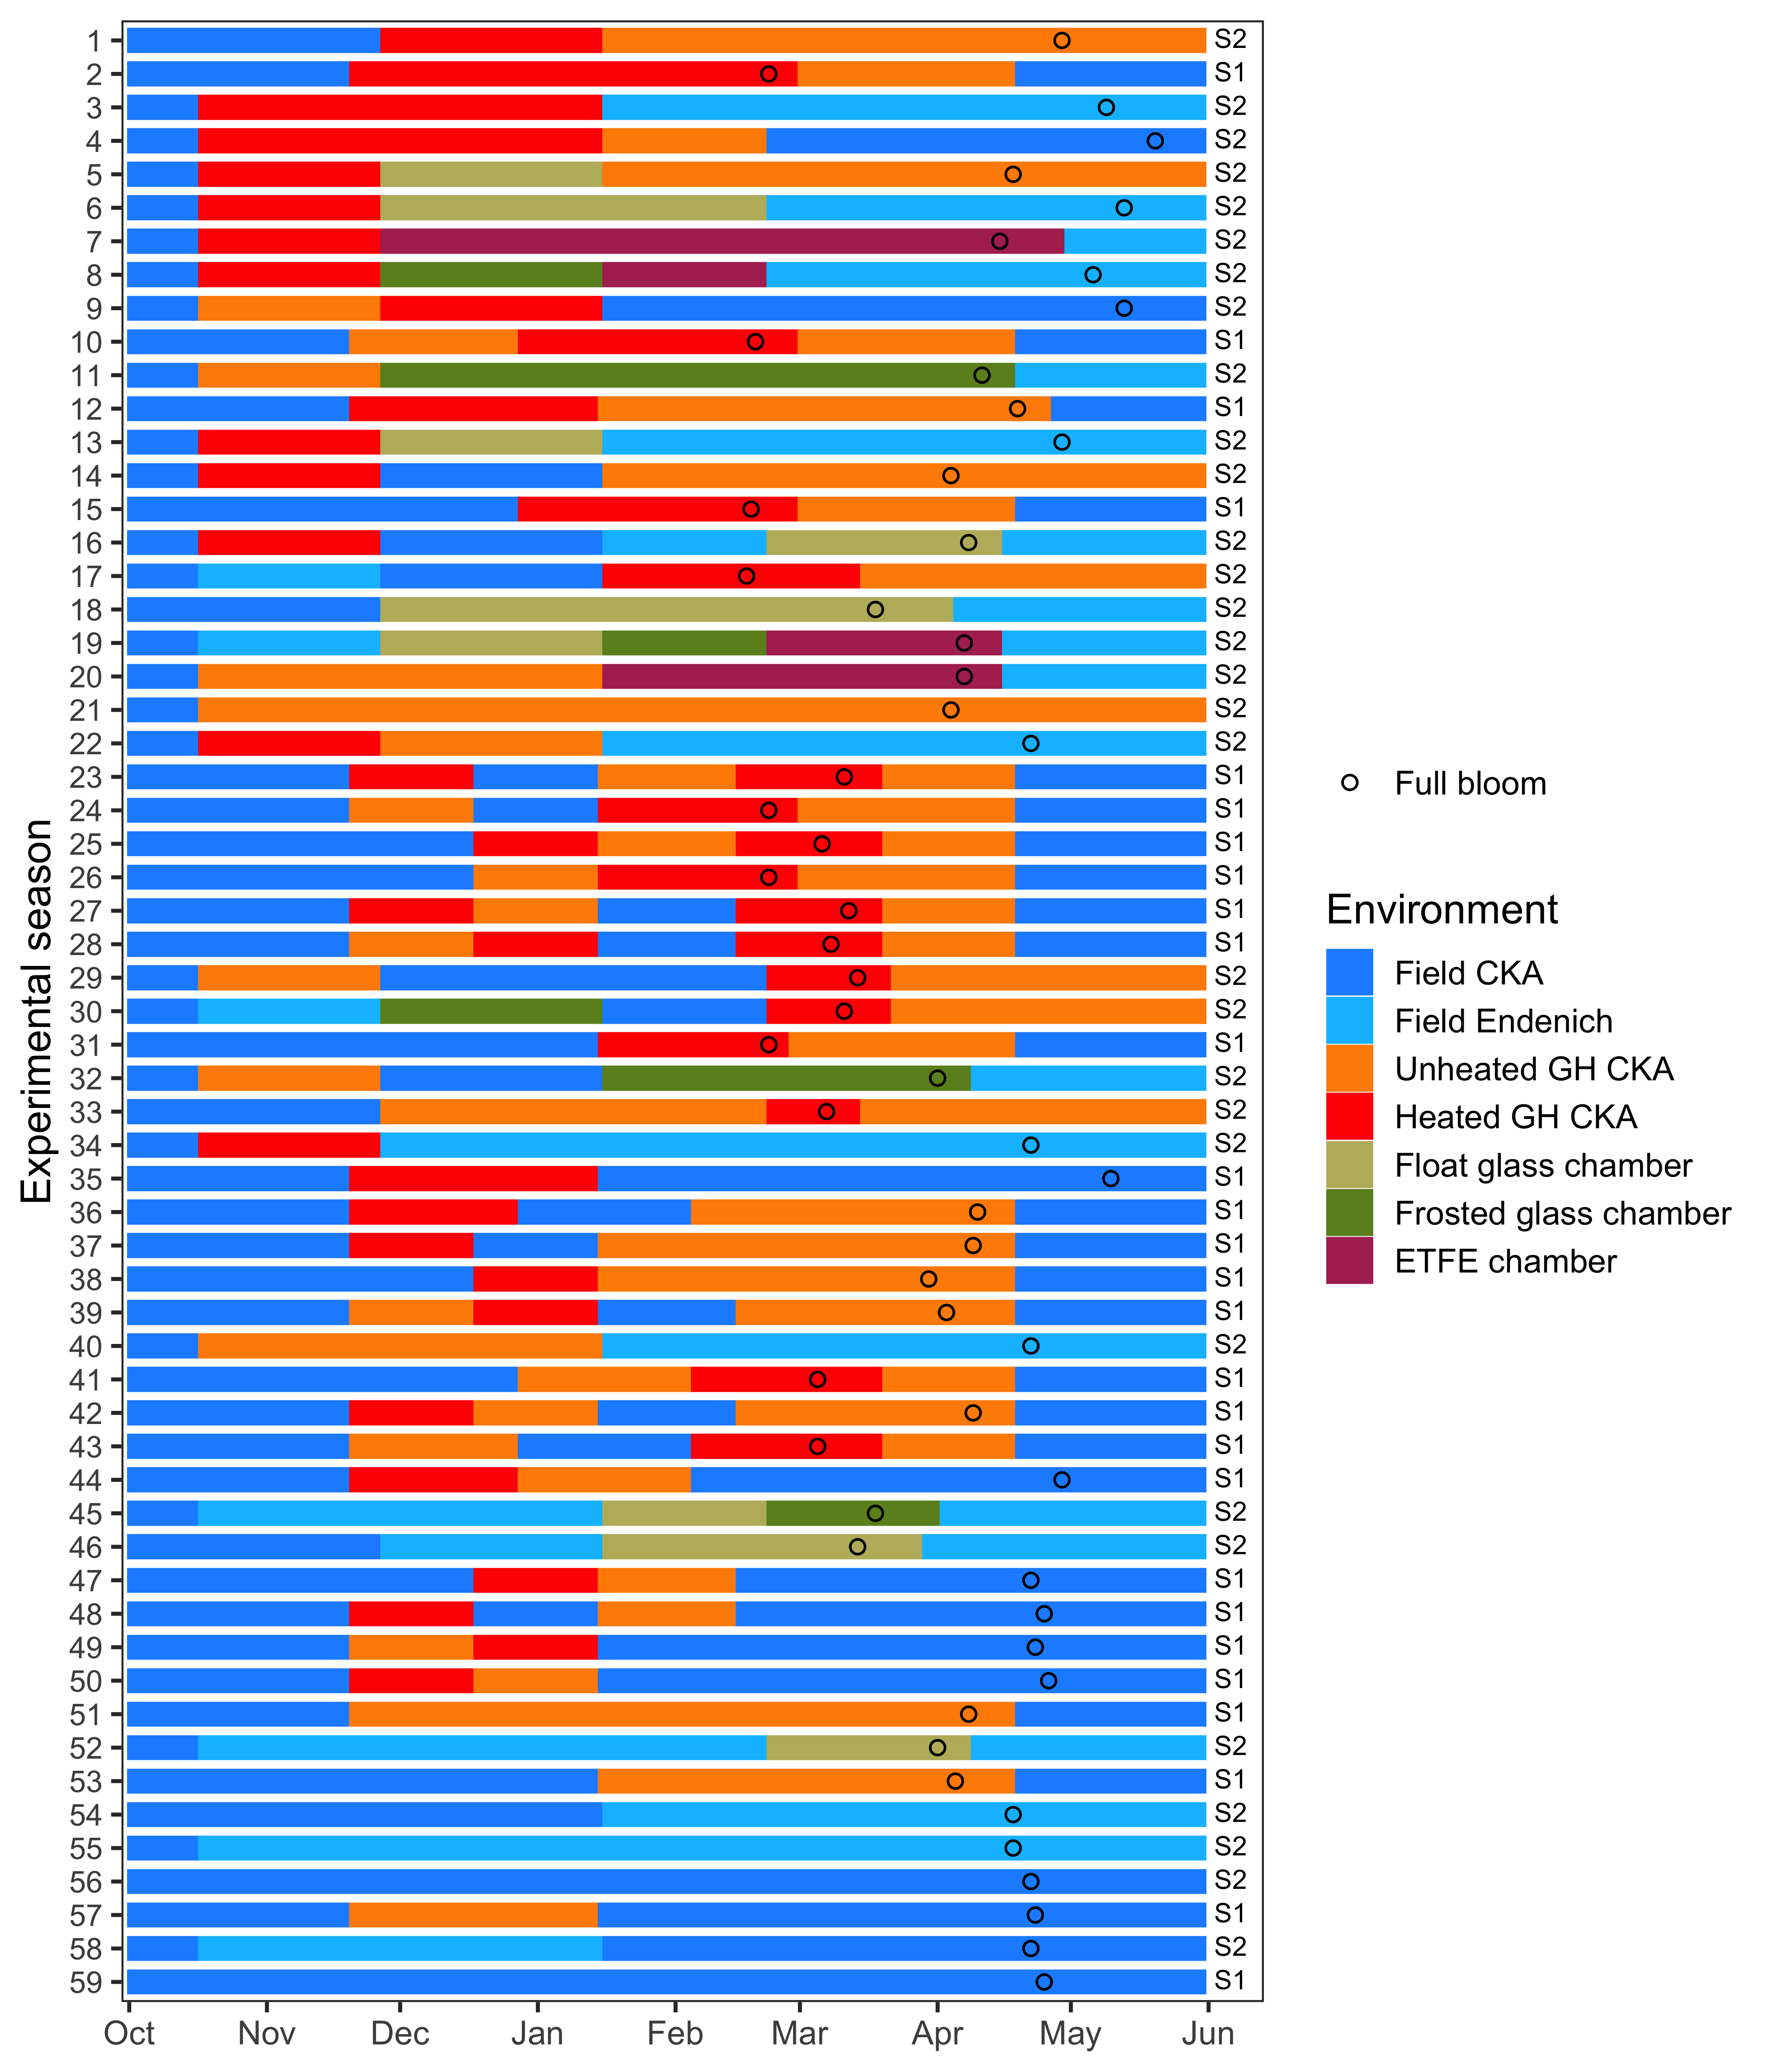
\includegraphics[height=0.71\textheight]{figures/supplementary_conditions} 

}

\caption{Experimental seasons used in the study. The first 5 experimental seasons represent the marginal experimental seasons excluded in the respective version of the analysis (see main manuscript for further details). In the 'Environment' legend, CKA stands for Campus Klein-Altendorf and ETFE stands for ethylene-tetrafluoroethylenecopolymer}\label{fig:fig_s2}
\end{figure}

The experimental setup allowed us to generate a substantial temperature
variation during the two winter seasons as well as conditions that may
have been marginal for apple trees to overcome dormancy as discussed in
the main manuscript. Most of the time, the mean temperature in those 5
marginal experimental seasons was in the upper part of the temperature
range identified among all experimental seasons (Fig. S3).

\newpage

\begin{figure}

{\centering 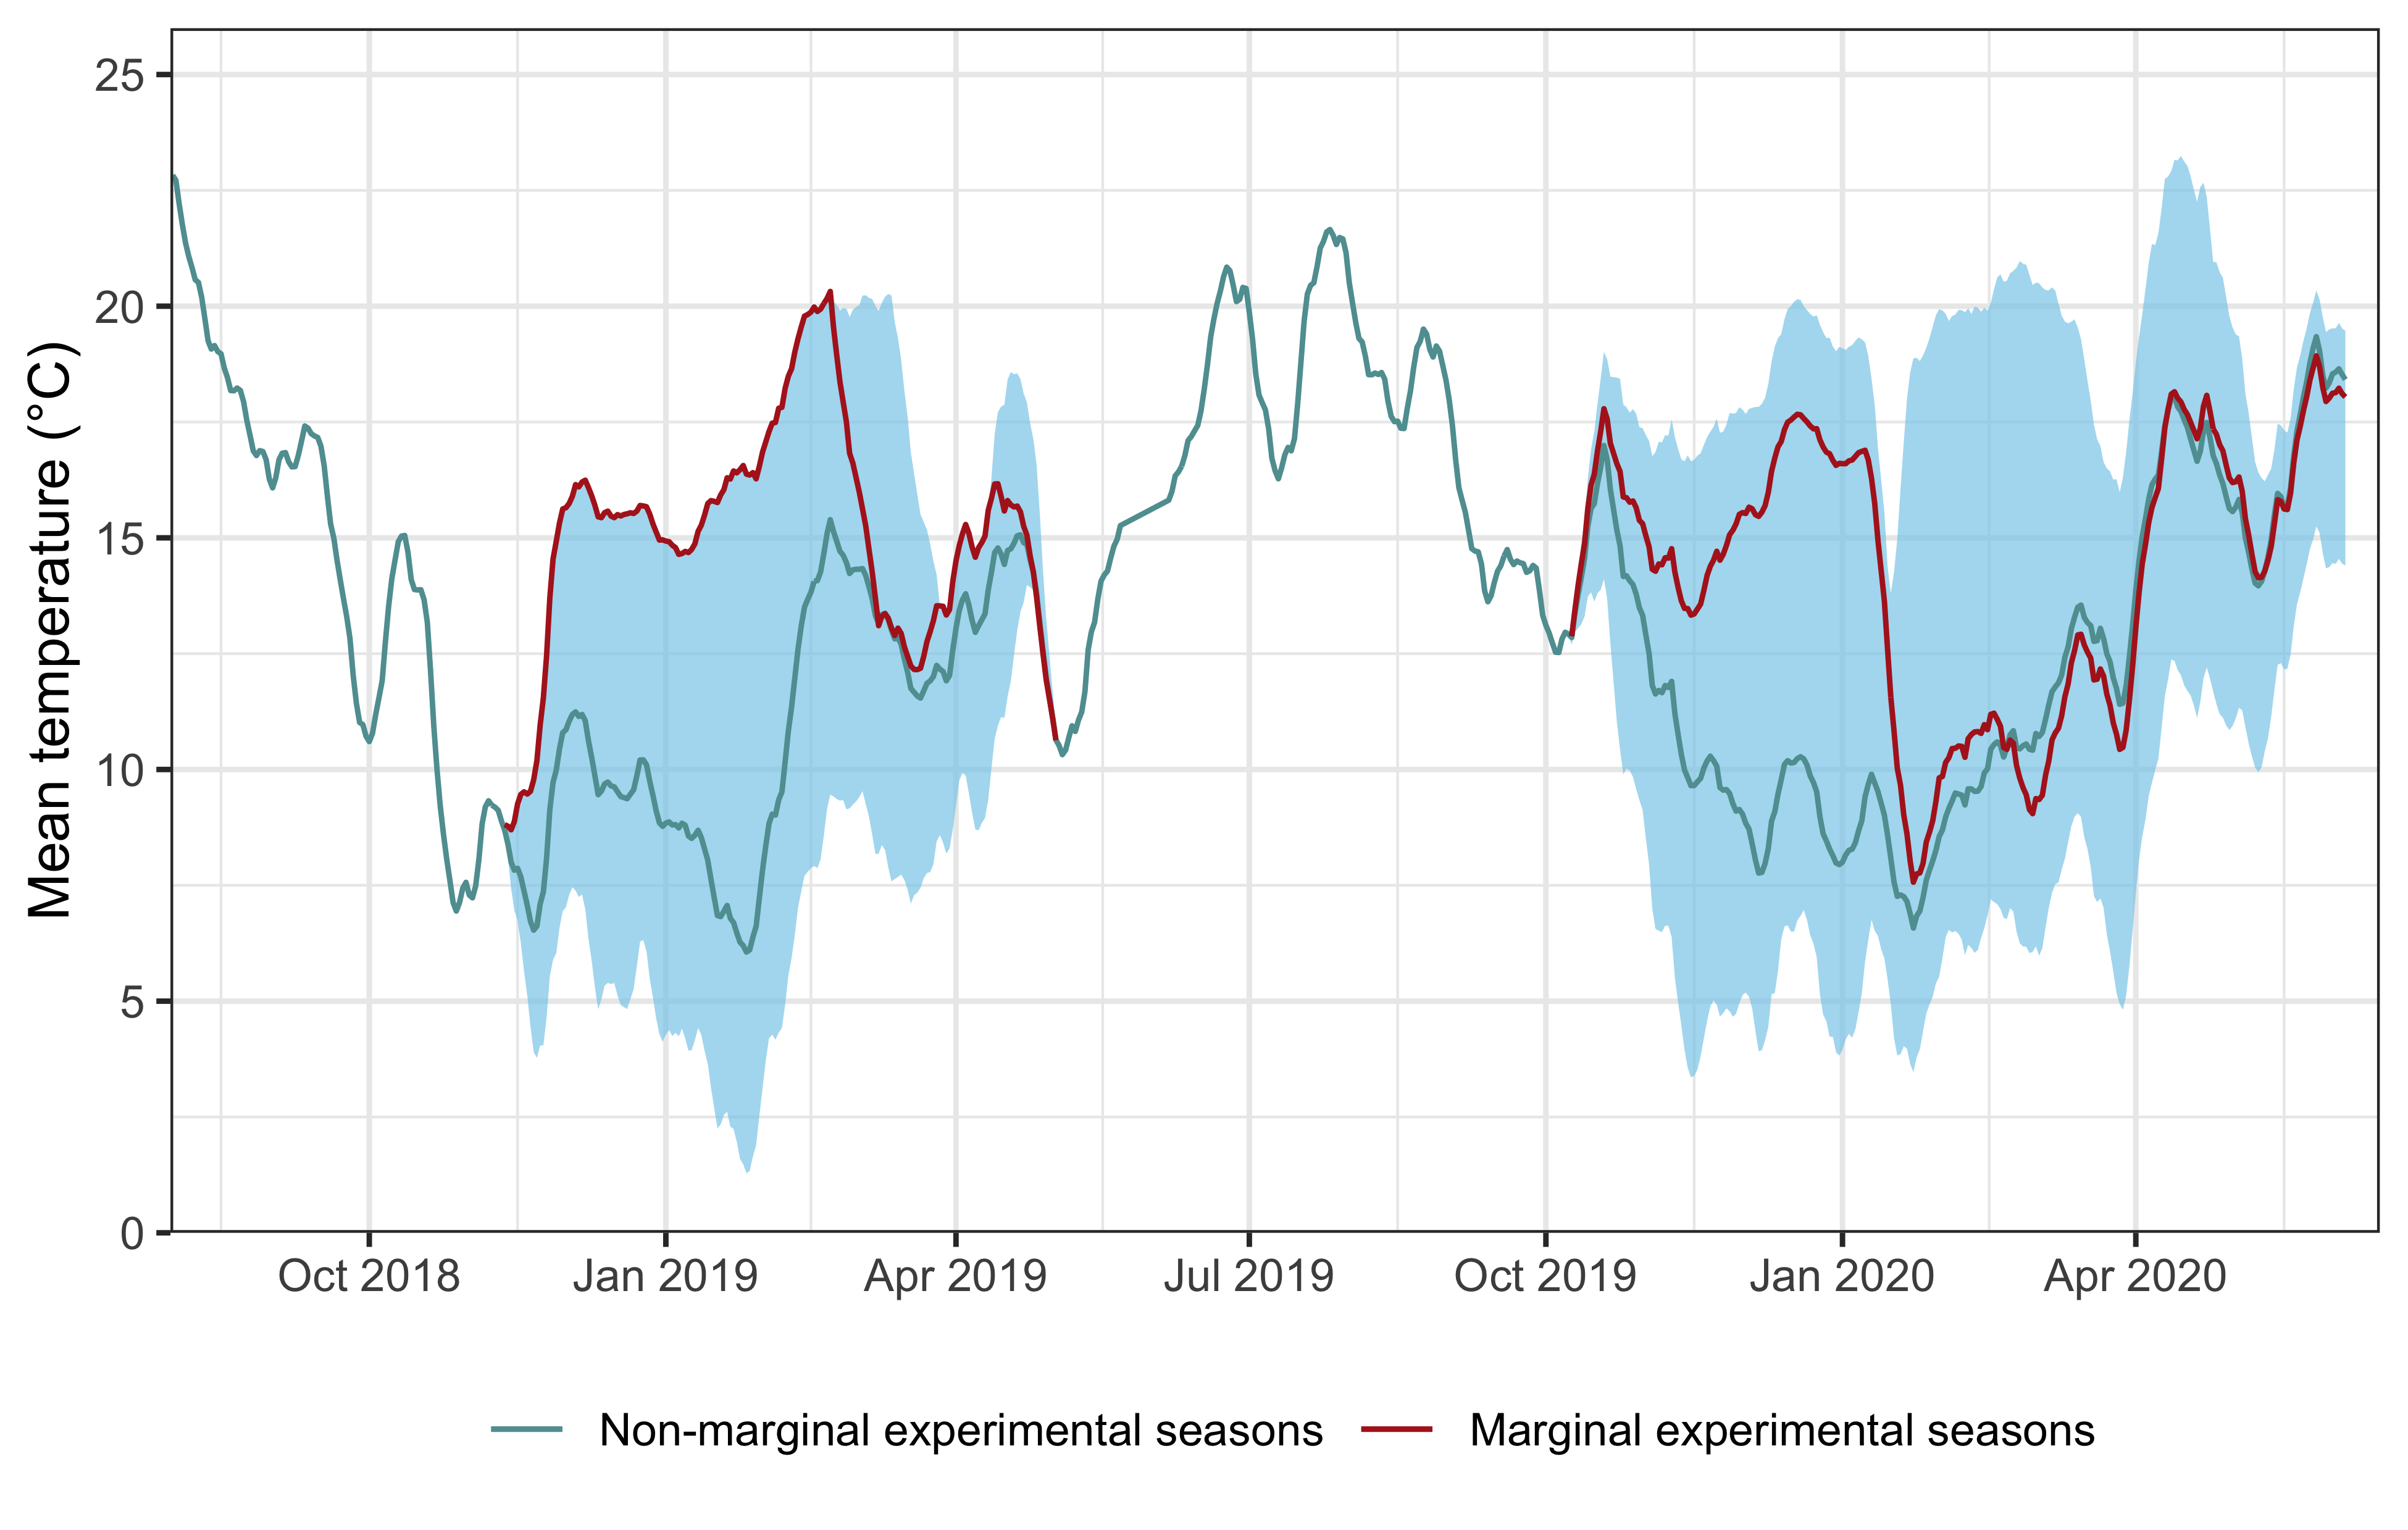
\includegraphics[width=0.9\linewidth]{figures/supplementary_conditions_2} 

}

\caption{Temperature variation among the experimental seasons used in this study. Whereas the solid red line in the plot shows the mean temperature among marginal experimental seasons (1 in the winter of 2018/2019 and 4 in the winter of 2019/2020), the blue solid line represents the mean temperature among all available experimental seasons (i.e. 59)}\label{fig:fig_s3}
\end{figure}

\hypertarget{parameters-used-in-each-model-run}{%
\section{Parameters used in each model
run}\label{parameters-used-in-each-model-run}}

The \texttt{phenologyFitter()} function from the \texttt{chillR} package
(Luedeling 2021), which is needed to fit the 12 model parameters to
data, requires an estimated set of parameters (i.e.~\texttt{par.guess})
as well as the \texttt{lower} and \texttt{upper} bounds for these
values. We initialized the model fitting procedure with a common set of
parameters for both versions of the analysis
(i.e.~PhenoFlex\textsubscript{all} and
PhenoFlex\textsubscript{excluded}).

\hypertarget{first-model-run}{%
\subsection{First model run}\label{first-model-run}}

\begin{Shaded}
\begin{Highlighting}[]
\CommentTok{\# Set the initial parameters (wide ranges)}
\CommentTok{\# Parameter \textless{}{-} c(yc,  zc,  s1, Tu,     E0,      E1,     A0,         A1,  Tf, Tc, Tb, slope)}
\NormalTok{lower       }\OtherTok{\textless{}{-}} \FunctionTok{c}\NormalTok{(}\DecValTok{20}\NormalTok{, }\DecValTok{100}\NormalTok{, }\FloatTok{0.1}\NormalTok{,  }\DecValTok{0}\NormalTok{, }\FloatTok{3000.0}\NormalTok{,  }\FloatTok{9000.0}\NormalTok{, }\FloatTok{6000.0}\NormalTok{,   }\FloatTok{5.00e+13}\NormalTok{,   }\DecValTok{0}\NormalTok{,  }\DecValTok{0}\NormalTok{,  }\DecValTok{0}\NormalTok{,  }\FloatTok{0.05}\NormalTok{)}
\NormalTok{par.guess   }\OtherTok{\textless{}{-}} \FunctionTok{c}\NormalTok{(}\DecValTok{40}\NormalTok{, }\DecValTok{190}\NormalTok{, }\FloatTok{0.5}\NormalTok{, }\DecValTok{25}\NormalTok{, }\FloatTok{3372.8}\NormalTok{,  }\FloatTok{9900.3}\NormalTok{, }\FloatTok{6319.5}\NormalTok{,   }\FloatTok{5.94e+13}\NormalTok{,   }\DecValTok{4}\NormalTok{, }\DecValTok{36}\NormalTok{,  }\DecValTok{4}\NormalTok{,  }\FloatTok{1.60}\NormalTok{)}
\NormalTok{upper       }\OtherTok{\textless{}{-}} \FunctionTok{c}\NormalTok{(}\DecValTok{80}\NormalTok{, }\DecValTok{500}\NormalTok{, }\FloatTok{1.0}\NormalTok{, }\DecValTok{30}\NormalTok{, }\FloatTok{4000.0}\NormalTok{, }\FloatTok{10000.0}\NormalTok{, }\FloatTok{7000.0}\NormalTok{,   }\FloatTok{6.00e+13}\NormalTok{,  }\DecValTok{10}\NormalTok{, }\DecValTok{40}\NormalTok{, }\DecValTok{10}\NormalTok{, }\FloatTok{50.00}\NormalTok{)}
\end{Highlighting}
\end{Shaded}

We introduced these parameters to the fitter function for each version
of the analysis. Note that the specific values for the parameters and
all scripts developed in this study are deposited in a public online
repository
\href{https://github.com/EduardoFernandezC/phenoflex_exp_data}{(https://github.com/EduardoFernandezC/phenoflex\_exp\_data)}.
The first fitting procedure resulted in \texttt{RMSE} values of 7.2 days
for PhenoFlex\textsubscript{all} and 4.13 days for
PhenoFlex\textsubscript{excluded}. In the second round of the fitting
procedure, we adjusted the parameter inputs.

\hypertarget{second-model-run}{%
\subsection{Second model run}\label{second-model-run}}

\begin{Shaded}
\begin{Highlighting}[]
\CommentTok{\# Set the parameters using the results from the previous run}

\CommentTok{\# Version PhenoFlex\_all (pheno\_fit\_v1\_r1$model\_fit$par)}
\CommentTok{\# Parameter \textless{}{-} c(yc,  zc,   s1,   Tu,     E0,      E1,     A0,       A1,   Tf,   Tc,  Tb, slope)}
\NormalTok{lower\_v1\_r2 }\OtherTok{\textless{}{-}} \FunctionTok{c}\NormalTok{(}\DecValTok{45}\NormalTok{, }\DecValTok{290}\NormalTok{, }\FloatTok{0.00}\NormalTok{, }\FloatTok{18.0}\NormalTok{, }\FloatTok{3000.0}\NormalTok{,  }\FloatTok{9000.0}\NormalTok{, }\FloatTok{6000.0}\NormalTok{, }\FloatTok{5.20e+13}\NormalTok{,  }\FloatTok{0.0}\NormalTok{, }\FloatTok{29.0}\NormalTok{,  }\FloatTok{0.0}\NormalTok{,  }\FloatTok{0.05}\NormalTok{)}
\NormalTok{par\_v1\_r2   }\OtherTok{\textless{}{-}} \FunctionTok{c}\NormalTok{(}\DecValTok{59}\NormalTok{, }\DecValTok{326}\NormalTok{, }\FloatTok{0.16}\NormalTok{, }\FloatTok{22.5}\NormalTok{, }\FloatTok{3309.9}\NormalTok{,  }\FloatTok{9900.1}\NormalTok{, }\FloatTok{6295.7}\NormalTok{, }\FloatTok{5.94e+13}\NormalTok{,  }\FloatTok{6.1}\NormalTok{, }\FloatTok{39.9}\NormalTok{,  }\FloatTok{8.6}\NormalTok{, }\FloatTok{14.60}\NormalTok{)}
\NormalTok{upper\_v1\_r2 }\OtherTok{\textless{}{-}} \FunctionTok{c}\NormalTok{(}\DecValTok{65}\NormalTok{, }\DecValTok{380}\NormalTok{, }\FloatTok{0.50}\NormalTok{, }\FloatTok{30.0}\NormalTok{, }\FloatTok{4000.0}\NormalTok{, }\FloatTok{10000.0}\NormalTok{, }\FloatTok{7000.0}\NormalTok{, }\FloatTok{6.20e+13}\NormalTok{, }\FloatTok{10.0}\NormalTok{, }\FloatTok{44.0}\NormalTok{, }\FloatTok{12.0}\NormalTok{, }\FloatTok{30.00}\NormalTok{)}


\CommentTok{\# Same for version PhenoFlex\_excluded (pheno\_fit\_v2\_r1$model\_fit$par)}
\CommentTok{\# Parameter \textless{}{-} c(yc,  zc,   s1,   Tu,     E0,      E1,     A0,       A1,   Tf,   Tc,   Tb, slope)}
\NormalTok{lower\_v2\_r2 }\OtherTok{\textless{}{-}} \FunctionTok{c}\NormalTok{(}\DecValTok{25}\NormalTok{, }\DecValTok{340}\NormalTok{, }\FloatTok{0.00}\NormalTok{, }\FloatTok{17.0}\NormalTok{, }\FloatTok{3000.0}\NormalTok{,  }\FloatTok{9000.0}\NormalTok{, }\FloatTok{6000.0}\NormalTok{, }\FloatTok{5.20e+13}\NormalTok{,  }\FloatTok{0.0}\NormalTok{, }\FloatTok{30.0}\NormalTok{,  }\FloatTok{0.0}\NormalTok{,  }\FloatTok{1.00}\NormalTok{)}
\NormalTok{par\_v2\_r2   }\OtherTok{\textless{}{-}} \FunctionTok{c}\NormalTok{(}\DecValTok{35}\NormalTok{, }\DecValTok{387}\NormalTok{, }\FloatTok{0.03}\NormalTok{, }\FloatTok{21.8}\NormalTok{, }\FloatTok{3371.0}\NormalTok{,  }\FloatTok{9900.8}\NormalTok{, }\FloatTok{6283.6}\NormalTok{, }\FloatTok{5.94e+13}\NormalTok{,  }\FloatTok{5.1}\NormalTok{, }\FloatTok{40.0}\NormalTok{,  }\FloatTok{6.3}\NormalTok{, }\FloatTok{40.00}\NormalTok{)}
\NormalTok{upper\_v2\_r2 }\OtherTok{\textless{}{-}} \FunctionTok{c}\NormalTok{(}\DecValTok{40}\NormalTok{, }\DecValTok{420}\NormalTok{, }\FloatTok{0.50}\NormalTok{, }\FloatTok{32.0}\NormalTok{, }\FloatTok{4000.0}\NormalTok{, }\FloatTok{10000.0}\NormalTok{, }\FloatTok{7000.0}\NormalTok{, }\FloatTok{6.20e+13}\NormalTok{, }\FloatTok{10.0}\NormalTok{, }\FloatTok{42.0}\NormalTok{, }\FloatTok{10.0}\NormalTok{, }\FloatTok{50.00}\NormalTok{)}
\end{Highlighting}
\end{Shaded}

In the second round of the fitting procedure,
PhenoFlex\textsubscript{all} reached an \texttt{RMSE} of 6.94 days,
whereas PhenoFlex\textsubscript{excluded} reached an \texttt{RMSE} of
3.91 days. In the third round of the fitting procedure, we adjusted the
parameter inputs as follow:

\hypertarget{third-model-run}{%
\subsection{Third model run}\label{third-model-run}}

\begin{Shaded}
\begin{Highlighting}[]
\CommentTok{\# Set the parameters using the results from the previous run}

\CommentTok{\# Version PhenoFlex\_all (pheno\_fit\_v1\_r2$model\_fit$par)}
\CommentTok{\# Parameter \textless{}{-} c(yc, zc,    s1,   Tu,     E0,      E1,     A0,       A1,   Tf,   Tc,   Tb, slope)}
\NormalTok{lower\_v1\_r3 }\OtherTok{\textless{}{-}} \FunctionTok{c}\NormalTok{(}\DecValTok{48}\NormalTok{, }\DecValTok{290}\NormalTok{, }\FloatTok{0.00}\NormalTok{, }\FloatTok{15.0}\NormalTok{, }\FloatTok{3000.0}\NormalTok{,  }\FloatTok{9000.0}\NormalTok{, }\FloatTok{6000.0}\NormalTok{, }\FloatTok{5.20e+13}\NormalTok{,  }\FloatTok{0.0}\NormalTok{, }\FloatTok{24.0}\NormalTok{,  }\FloatTok{0.0}\NormalTok{,  }\FloatTok{0.05}\NormalTok{)}
\NormalTok{par\_v1\_r3   }\OtherTok{\textless{}{-}} \FunctionTok{c}\NormalTok{(}\DecValTok{58}\NormalTok{, }\DecValTok{332}\NormalTok{, }\FloatTok{0.39}\NormalTok{, }\FloatTok{22.1}\NormalTok{, }\FloatTok{3310.5}\NormalTok{,  }\FloatTok{9900.3}\NormalTok{, }\FloatTok{6344.8}\NormalTok{, }\FloatTok{5.94e+13}\NormalTok{,  }\FloatTok{7.2}\NormalTok{, }\FloatTok{35.0}\NormalTok{,  }\FloatTok{8.8}\NormalTok{, }\FloatTok{18.20}\NormalTok{)}
\NormalTok{upper\_v1\_r3 }\OtherTok{\textless{}{-}} \FunctionTok{c}\NormalTok{(}\DecValTok{68}\NormalTok{, }\DecValTok{370}\NormalTok{, }\FloatTok{0.65}\NormalTok{, }\FloatTok{32.0}\NormalTok{, }\FloatTok{4000.0}\NormalTok{, }\FloatTok{10500.0}\NormalTok{, }\FloatTok{7000.0}\NormalTok{, }\FloatTok{6.20e+13}\NormalTok{, }\FloatTok{11.0}\NormalTok{, }\FloatTok{44.0}\NormalTok{, }\FloatTok{11.0}\NormalTok{, }\FloatTok{35.00}\NormalTok{)}


\CommentTok{\# Same for PhenoFlex\_excluded (pheno\_fit\_v2\_r2$model\_fit$par)}
\CommentTok{\# Parameter \textless{}{-} c(yc, zc,    s1,   Tu,     E0,      E1,     A0,       A1,   Tf,   Tc,   Tb, slope)}
\NormalTok{lower\_v2\_r3 }\OtherTok{\textless{}{-}} \FunctionTok{c}\NormalTok{(}\DecValTok{20}\NormalTok{, }\DecValTok{350}\NormalTok{, }\FloatTok{0.00}\NormalTok{, }\FloatTok{18.0}\NormalTok{, }\FloatTok{3000.0}\NormalTok{,  }\FloatTok{9000.0}\NormalTok{, }\FloatTok{6000.0}\NormalTok{, }\FloatTok{5.20e+13}\NormalTok{,  }\FloatTok{0.0}\NormalTok{, }\FloatTok{30.0}\NormalTok{,  }\FloatTok{0.0}\NormalTok{,  }\FloatTok{1.00}\NormalTok{)}
\NormalTok{par\_v2\_r3   }\OtherTok{\textless{}{-}} \FunctionTok{c}\NormalTok{(}\DecValTok{34}\NormalTok{, }\DecValTok{406}\NormalTok{, }\FloatTok{0.20}\NormalTok{, }\FloatTok{21.4}\NormalTok{, }\FloatTok{3371.4}\NormalTok{,  }\FloatTok{9901.3}\NormalTok{, }\FloatTok{6214.0}\NormalTok{, }\FloatTok{5.94e+13}\NormalTok{,  }\FloatTok{1.5}\NormalTok{, }\FloatTok{42.0}\NormalTok{,  }\FloatTok{6.1}\NormalTok{, }\FloatTok{10.70}\NormalTok{)}
\NormalTok{upper\_v2\_r3 }\OtherTok{\textless{}{-}} \FunctionTok{c}\NormalTok{(}\DecValTok{50}\NormalTok{, }\DecValTok{450}\NormalTok{, }\FloatTok{0.55}\NormalTok{, }\FloatTok{35.0}\NormalTok{, }\FloatTok{4000.0}\NormalTok{, }\FloatTok{10500.0}\NormalTok{, }\FloatTok{7000.0}\NormalTok{, }\FloatTok{6.20e+13}\NormalTok{, }\FloatTok{10.0}\NormalTok{, }\FloatTok{46.0}\NormalTok{, }\FloatTok{10.0}\NormalTok{, }\FloatTok{35.00}\NormalTok{)}
\end{Highlighting}
\end{Shaded}

After the third round of the fitting procedure, \texttt{RMSE} values
decreased to 6.63 days for PhenoFlex\textsubscript{all} and 3.91 days
for PhenoFlex\textsubscript{excluded}. In the fourth round of the
fitting procedure, we used the following set of parameters:

\hypertarget{fourth-model-run}{%
\subsection{Fourth model run}\label{fourth-model-run}}

\begin{Shaded}
\begin{Highlighting}[]
\CommentTok{\# Set the parameters using the results from the previous run}

\CommentTok{\# Version PhenoFlex\_all (pheno\_fit\_v1\_r3$model\_fit$par)}
\CommentTok{\# Parameter \textless{}{-} c(yc,  zc,   s1,   Tu,     E0,      E1,     A0,       A1,   Tf,   Tc,   Tb, slope)}
\NormalTok{lower\_v1\_r4 }\OtherTok{\textless{}{-}} \FunctionTok{c}\NormalTok{(}\DecValTok{45}\NormalTok{, }\DecValTok{290}\NormalTok{, }\FloatTok{0.00}\NormalTok{, }\FloatTok{15.0}\NormalTok{, }\FloatTok{3000.0}\NormalTok{,  }\FloatTok{9000.0}\NormalTok{, }\FloatTok{5500.0}\NormalTok{, }\FloatTok{5.20e+13}\NormalTok{,  }\FloatTok{0.0}\NormalTok{, }\FloatTok{20.0}\NormalTok{,  }\FloatTok{0.0}\NormalTok{,  }\FloatTok{1.00}\NormalTok{)}
\NormalTok{par\_v1\_r4   }\OtherTok{\textless{}{-}} \FunctionTok{c}\NormalTok{(}\DecValTok{60}\NormalTok{, }\DecValTok{339}\NormalTok{, }\FloatTok{0.54}\NormalTok{, }\FloatTok{23.0}\NormalTok{, }\FloatTok{3310.3}\NormalTok{,  }\FloatTok{9901.5}\NormalTok{, }\FloatTok{6346.3}\NormalTok{, }\FloatTok{5.94e+13}\NormalTok{,  }\FloatTok{7.2}\NormalTok{, }\FloatTok{30.7}\NormalTok{,  }\FloatTok{7.6}\NormalTok{,  }\FloatTok{7.30}\NormalTok{)}
\NormalTok{upper\_v1\_r4 }\OtherTok{\textless{}{-}} \FunctionTok{c}\NormalTok{(}\DecValTok{70}\NormalTok{, }\DecValTok{370}\NormalTok{, }\FloatTok{0.75}\NormalTok{, }\FloatTok{32.0}\NormalTok{, }\FloatTok{4000.0}\NormalTok{, }\FloatTok{10300.0}\NormalTok{, }\FloatTok{7000.0}\NormalTok{, }\FloatTok{6.20e+13}\NormalTok{, }\FloatTok{12.0}\NormalTok{, }\FloatTok{40.0}\NormalTok{, }\FloatTok{12.0}\NormalTok{, }\FloatTok{20.00}\NormalTok{)}


\CommentTok{\# Same for version 2 (pheno\_fit\_v2\_r3$model\_fit$par)}
\CommentTok{\# Parameter \textless{}{-} c(yc, zc,    s1,   Tu,     E0,      E1,     A0,       A1,   Tf,   Tc,   Tb, slope)}
\NormalTok{lower\_v2\_r4 }\OtherTok{\textless{}{-}} \FunctionTok{c}\NormalTok{(}\DecValTok{28}\NormalTok{, }\DecValTok{360}\NormalTok{, }\FloatTok{0.00}\NormalTok{, }\FloatTok{17.0}\NormalTok{, }\FloatTok{3000.0}\NormalTok{,  }\FloatTok{9300.0}\NormalTok{, }\FloatTok{5800.0}\NormalTok{, }\FloatTok{5.30e+13}\NormalTok{,  }\FloatTok{0.0}\NormalTok{, }\FloatTok{35.0}\NormalTok{,  }\FloatTok{0.0}\NormalTok{, }\FloatTok{10.00}\NormalTok{)}
\NormalTok{par\_v2\_r4   }\OtherTok{\textless{}{-}} \FunctionTok{c}\NormalTok{(}\DecValTok{34}\NormalTok{, }\DecValTok{396}\NormalTok{, }\FloatTok{0.20}\NormalTok{, }\FloatTok{21.6}\NormalTok{, }\FloatTok{3371.0}\NormalTok{,  }\FloatTok{9901.3}\NormalTok{, }\FloatTok{6214.0}\NormalTok{, }\FloatTok{5.94e+13}\NormalTok{,  }\FloatTok{1.5}\NormalTok{, }\FloatTok{46.0}\NormalTok{,  }\FloatTok{5.9}\NormalTok{, }\FloatTok{11.12}\NormalTok{)}
\NormalTok{upper\_v2\_r4 }\OtherTok{\textless{}{-}} \FunctionTok{c}\NormalTok{(}\DecValTok{44}\NormalTok{, }\DecValTok{440}\NormalTok{, }\FloatTok{0.45}\NormalTok{, }\FloatTok{30.0}\NormalTok{, }\FloatTok{4000.0}\NormalTok{, }\FloatTok{10500.0}\NormalTok{, }\FloatTok{6800.0}\NormalTok{, }\FloatTok{6.50e+13}\NormalTok{, }\FloatTok{10.0}\NormalTok{, }\FloatTok{48.0}\NormalTok{, }\FloatTok{12.0}\NormalTok{, }\FloatTok{40.00}\NormalTok{)}
\end{Highlighting}
\end{Shaded}

In this round of the fitting procedure, PhenoFlex\textsubscript{all}
reached an \texttt{RMSE} of 6.59 days, whereas
PhenoFlex\textsubscript{excluded} reached an \texttt{RMSE} of 3.65 days.

\hypertarget{fifth-model-run}{%
\subsection{Fifth model run}\label{fifth-model-run}}

\begin{Shaded}
\begin{Highlighting}[]
\CommentTok{\# Set the parameters using the results from the previous run}
\CommentTok{\# Version PhenoFlex\_all (pheno\_fit\_v1\_r4$model\_fit$par)}
\CommentTok{\# Parameter \textless{}{-} c(yc,  zc,   s1,   Tu,     E0,      E1,     A0,       A1,   Tf,   Tc,   Tb, slope)}
\NormalTok{lower\_v1\_r5 }\OtherTok{\textless{}{-}} \FunctionTok{c}\NormalTok{(}\DecValTok{50}\NormalTok{, }\DecValTok{330}\NormalTok{, }\FloatTok{0.00}\NormalTok{, }\FloatTok{18.0}\NormalTok{, }\FloatTok{3000.0}\NormalTok{,  }\FloatTok{9600.0}\NormalTok{, }\FloatTok{6000.0}\NormalTok{, }\FloatTok{5.50e+13}\NormalTok{,  }\FloatTok{2.0}\NormalTok{, }\FloatTok{30.0}\NormalTok{,  }\FloatTok{2.0}\NormalTok{,  }\FloatTok{0.50}\NormalTok{)}
\NormalTok{par\_v1\_r5   }\OtherTok{\textless{}{-}} \FunctionTok{c}\NormalTok{(}\DecValTok{60}\NormalTok{, }\DecValTok{354}\NormalTok{, }\FloatTok{0.47}\NormalTok{, }\FloatTok{22.8}\NormalTok{, }\FloatTok{3310.3}\NormalTok{,  }\FloatTok{9901.5}\NormalTok{, }\FloatTok{6344.3}\NormalTok{, }\FloatTok{5.94e+13}\NormalTok{,  }\FloatTok{7.2}\NormalTok{, }\FloatTok{36.0}\NormalTok{,  }\FloatTok{7.6}\NormalTok{,  }\FloatTok{7.63}\NormalTok{)}
\NormalTok{upper\_v1\_r5 }\OtherTok{\textless{}{-}} \FunctionTok{c}\NormalTok{(}\DecValTok{75}\NormalTok{, }\DecValTok{370}\NormalTok{, }\FloatTok{0.55}\NormalTok{, }\FloatTok{28.0}\NormalTok{, }\FloatTok{4000.0}\NormalTok{, }\FloatTok{10300.0}\NormalTok{, }\FloatTok{7000.0}\NormalTok{, }\FloatTok{6.50e+13}\NormalTok{, }\FloatTok{10.0}\NormalTok{, }\FloatTok{42.0}\NormalTok{, }\FloatTok{12.0}\NormalTok{, }\FloatTok{15.00}\NormalTok{)}


\CommentTok{\# Same for version PhenoFlex (pheno\_fit\_v2\_r4$model\_fit$par)}
\CommentTok{\# Parameter \textless{}{-} c(yc,  zc,   s1,   Tu,     E0,      E1,     A0,       A1,   Tf,   Tc,   Tb, slope)}
\NormalTok{lower\_v2\_r5 }\OtherTok{\textless{}{-}} \FunctionTok{c}\NormalTok{(}\DecValTok{27}\NormalTok{, }\DecValTok{360}\NormalTok{, }\FloatTok{0.00}\NormalTok{, }\FloatTok{18.0}\NormalTok{, }\FloatTok{3000.0}\NormalTok{,  }\FloatTok{9500.0}\NormalTok{, }\FloatTok{5800.0}\NormalTok{, }\FloatTok{5.50e+13}\NormalTok{,  }\FloatTok{0.0}\NormalTok{, }\FloatTok{35.0}\NormalTok{,  }\FloatTok{1.0}\NormalTok{,  }\FloatTok{1.00}\NormalTok{)}
\NormalTok{par\_v2\_r5   }\OtherTok{\textless{}{-}} \FunctionTok{c}\NormalTok{(}\DecValTok{34}\NormalTok{, }\DecValTok{383}\NormalTok{, }\FloatTok{0.21}\NormalTok{, }\FloatTok{22.5}\NormalTok{, }\FloatTok{3371.0}\NormalTok{,  }\FloatTok{9901.3}\NormalTok{, }\FloatTok{6213.9}\NormalTok{, }\FloatTok{5.94e+13}\NormalTok{,  }\FloatTok{1.5}\NormalTok{, }\FloatTok{45.6}\NormalTok{,  }\FloatTok{5.9}\NormalTok{,  }\FloatTok{1.08}\NormalTok{)}
\NormalTok{upper\_v2\_r5 }\OtherTok{\textless{}{-}} \FunctionTok{c}\NormalTok{(}\DecValTok{37}\NormalTok{, }\DecValTok{400}\NormalTok{, }\FloatTok{0.55}\NormalTok{, }\FloatTok{32.0}\NormalTok{, }\FloatTok{4000.0}\NormalTok{, }\FloatTok{10300.0}\NormalTok{, }\FloatTok{6800.0}\NormalTok{, }\FloatTok{6.30e+13}\NormalTok{,  }\FloatTok{8.0}\NormalTok{, }\FloatTok{48.0}\NormalTok{, }\FloatTok{10.0}\NormalTok{, }\FloatTok{25.00}\NormalTok{)}
\end{Highlighting}
\end{Shaded}

In this round of the fitting procedure, PhenoFlex\textsubscript{all}
reached an \texttt{RMSE} of 6.57 days, whereas
PhenoFlex\textsubscript{excluded} reached an \texttt{RMSE} of 3.56 days.

\hypertarget{sixth-model-run}{%
\subsection{Sixth model run}\label{sixth-model-run}}

\begin{Shaded}
\begin{Highlighting}[]
\CommentTok{\# Set the parameters using the results from the previous run}
\CommentTok{\# Version PhenoFlex\_all (pheno\_fit\_v1\_r5$model\_fit$par)}
\CommentTok{\# Parameter \textless{}{-} c(yc,  zc,   s1,   Tu,     E0,      E1,     A0,       A1,   Tf,   Tc,   Tb, slope)}
\NormalTok{lower\_v1\_r6 }\OtherTok{\textless{}{-}} \FunctionTok{c}\NormalTok{(}\DecValTok{40}\NormalTok{, }\DecValTok{290}\NormalTok{, }\FloatTok{0.00}\NormalTok{, }\FloatTok{18.0}\NormalTok{, }\FloatTok{2900.0}\NormalTok{,  }\FloatTok{9000.0}\NormalTok{, }\FloatTok{5700.0}\NormalTok{, }\FloatTok{5.30e+13}\NormalTok{,  }\FloatTok{0.0}\NormalTok{, }\FloatTok{20.0}\NormalTok{,  }\FloatTok{0.0}\NormalTok{,  }\FloatTok{0.01}\NormalTok{)}
\NormalTok{par\_v1\_r6   }\OtherTok{\textless{}{-}} \FunctionTok{c}\NormalTok{(}\DecValTok{60}\NormalTok{, }\DecValTok{343}\NormalTok{, }\FloatTok{0.32}\NormalTok{, }\FloatTok{25.1}\NormalTok{, }\FloatTok{3310.3}\NormalTok{,  }\FloatTok{9901.6}\NormalTok{, }\FloatTok{6342.9}\NormalTok{, }\FloatTok{5.94e+13}\NormalTok{,  }\FloatTok{5.6}\NormalTok{, }\FloatTok{33.6}\NormalTok{,  }\FloatTok{7.0}\NormalTok{,  }\FloatTok{2.24}\NormalTok{)}
\NormalTok{upper\_v1\_r6 }\OtherTok{\textless{}{-}} \FunctionTok{c}\NormalTok{(}\DecValTok{80}\NormalTok{, }\DecValTok{390}\NormalTok{, }\FloatTok{0.55}\NormalTok{, }\FloatTok{32.0}\NormalTok{, }\FloatTok{3900.0}\NormalTok{, }\FloatTok{10500.0}\NormalTok{, }\FloatTok{6900.0}\NormalTok{, }\FloatTok{6.80e+13}\NormalTok{, }\FloatTok{12.0}\NormalTok{, }\FloatTok{48.0}\NormalTok{, }\FloatTok{12.0}\NormalTok{, }\FloatTok{20.00}\NormalTok{)}


\CommentTok{\# Same for version PhenoFlex\_excluded (pheno\_fit\_v2\_r5$model\_fit$par)}
\CommentTok{\# Parameter \textless{}{-} c(yc,  zc,   s1,   Tu,     E0,      E1,     A0,       A1,   Tf,   Tc,   Tb, slope)}
\NormalTok{lower\_v2\_r6 }\OtherTok{\textless{}{-}} \FunctionTok{c}\NormalTok{(}\DecValTok{25}\NormalTok{, }\DecValTok{330}\NormalTok{, }\FloatTok{0.00}\NormalTok{, }\FloatTok{18.0}\NormalTok{, }\FloatTok{3000.0}\NormalTok{,  }\FloatTok{9200.0}\NormalTok{, }\FloatTok{5700.0}\NormalTok{, }\FloatTok{5.40e+13}\NormalTok{,  }\FloatTok{0.05}\NormalTok{, }\FloatTok{40.0}\NormalTok{,  }\FloatTok{0.0}\NormalTok{,  }\FloatTok{0.50}\NormalTok{)}
\NormalTok{par\_v2\_r6   }\OtherTok{\textless{}{-}} \FunctionTok{c}\NormalTok{(}\DecValTok{35}\NormalTok{, }\DecValTok{361}\NormalTok{, }\FloatTok{0.15}\NormalTok{, }\FloatTok{22.4}\NormalTok{, }\FloatTok{3371.0}\NormalTok{,  }\FloatTok{9901.3}\NormalTok{, }\FloatTok{6213.8}\NormalTok{, }\FloatTok{5.94e+13}\NormalTok{,  }\FloatTok{1.45}\NormalTok{, }\FloatTok{48.0}\NormalTok{,  }\FloatTok{5.9}\NormalTok{,  }\FloatTok{1.10}\NormalTok{)}
\NormalTok{upper\_v2\_r6 }\OtherTok{\textless{}{-}} \FunctionTok{c}\NormalTok{(}\DecValTok{40}\NormalTok{, }\DecValTok{390}\NormalTok{, }\FloatTok{0.35}\NormalTok{, }\FloatTok{30.0}\NormalTok{, }\FloatTok{4000.0}\NormalTok{, }\FloatTok{10800.0}\NormalTok{, }\FloatTok{6900.0}\NormalTok{, }\FloatTok{6.60e+13}\NormalTok{, }\FloatTok{10.00}\NormalTok{, }\FloatTok{50.0}\NormalTok{, }\FloatTok{10.0}\NormalTok{, }\FloatTok{20.00}\NormalTok{)}
\end{Highlighting}
\end{Shaded}

In this round of the fitting procedure, PhenoFlex\textsubscript{all}
reached an \texttt{RMSE} of 6.41 days, whereas
PhenoFlex\textsubscript{excluded} reached an \texttt{RMSE} of 3.55 days.

\hypertarget{seventh-model-run}{%
\subsection{Seventh model run}\label{seventh-model-run}}

\begin{Shaded}
\begin{Highlighting}[]
\CommentTok{\# Set the parameters using the results from the previous run}
\CommentTok{\# Version PhenoFlex\_all (pheno\_fit\_v1\_r6$model\_fit$par)}
\CommentTok{\# Parameter \textless{}{-} c(yc,  zc,   s1,   Tu,     E0,      E1,     A0,       A1,   Tf,   Tc,   Tb, slope)}
\NormalTok{lower\_v1\_r7 }\OtherTok{\textless{}{-}} \FunctionTok{c}\NormalTok{(}\DecValTok{55}\NormalTok{, }\DecValTok{325}\NormalTok{, }\FloatTok{0.00}\NormalTok{, }\FloatTok{20.0}\NormalTok{, }\FloatTok{3000.0}\NormalTok{,  }\FloatTok{9000.0}\NormalTok{, }\FloatTok{5500.0}\NormalTok{, }\FloatTok{5.50e+13}\NormalTok{,  }\FloatTok{0.0}\NormalTok{, }\FloatTok{30.0}\NormalTok{,  }\FloatTok{2.0}\NormalTok{,  }\FloatTok{0.00}\NormalTok{)}
\NormalTok{par\_v1\_r7   }\OtherTok{\textless{}{-}} \FunctionTok{c}\NormalTok{(}\DecValTok{61}\NormalTok{, }\DecValTok{334}\NormalTok{, }\FloatTok{0.53}\NormalTok{, }\FloatTok{25.0}\NormalTok{, }\FloatTok{3310.3}\NormalTok{,  }\FloatTok{9901.6}\NormalTok{, }\FloatTok{6342.7}\NormalTok{, }\FloatTok{5.94e+13}\NormalTok{,  }\FloatTok{6.4}\NormalTok{, }\FloatTok{33.9}\NormalTok{,  }\FloatTok{7.0}\NormalTok{,  }\FloatTok{1.57}\NormalTok{)}
\NormalTok{upper\_v1\_r7 }\OtherTok{\textless{}{-}} \FunctionTok{c}\NormalTok{(}\DecValTok{65}\NormalTok{, }\DecValTok{345}\NormalTok{, }\FloatTok{0.65}\NormalTok{, }\FloatTok{30.0}\NormalTok{, }\FloatTok{4000.0}\NormalTok{, }\FloatTok{10500.0}\NormalTok{, }\FloatTok{6600.0}\NormalTok{, }\FloatTok{6.50e+13}\NormalTok{, }\FloatTok{10.0}\NormalTok{, }\FloatTok{40.0}\NormalTok{, }\FloatTok{10.0}\NormalTok{, }\FloatTok{10.00}\NormalTok{)}


\CommentTok{\# Same for version PhenoFlex\_excluded (pheno\_fit\_v2\_r6$model\_fit$par)}
\CommentTok{\# Parameter \textless{}{-} c(yc,  zc,   s1,   Tu,     E0,      E1,     A0,       A1,   Tf,   Tc,   Tb, slope)}
\NormalTok{lower\_v2\_r7 }\OtherTok{\textless{}{-}} \FunctionTok{c}\NormalTok{(}\DecValTok{30}\NormalTok{, }\DecValTok{365}\NormalTok{, }\FloatTok{0.000}\NormalTok{, }\FloatTok{20.0}\NormalTok{, }\FloatTok{3000.0}\NormalTok{,  }\FloatTok{9500.0}\NormalTok{, }\FloatTok{5800.0}\NormalTok{, }\FloatTok{5.50e+13}\NormalTok{,  }\FloatTok{0.0}\NormalTok{, }\FloatTok{35.0}\NormalTok{,  }\FloatTok{0.0}\NormalTok{,  }\FloatTok{1.00}\NormalTok{)}
\NormalTok{par\_v2\_r7   }\OtherTok{\textless{}{-}} \FunctionTok{c}\NormalTok{(}\DecValTok{34}\NormalTok{, }\DecValTok{380}\NormalTok{, }\FloatTok{0.160}\NormalTok{, }\FloatTok{26.4}\NormalTok{, }\FloatTok{3371.0}\NormalTok{,  }\FloatTok{9901.3}\NormalTok{, }\FloatTok{6214.2}\NormalTok{, }\FloatTok{5.94e+13}\NormalTok{,  }\FloatTok{1.3}\NormalTok{, }\FloatTok{41.2}\NormalTok{,  }\FloatTok{3.3}\NormalTok{,  }\FloatTok{1.12}\NormalTok{)}
\NormalTok{upper\_v2\_r7 }\OtherTok{\textless{}{-}} \FunctionTok{c}\NormalTok{(}\DecValTok{40}\NormalTok{, }\DecValTok{385}\NormalTok{, }\FloatTok{0.225}\NormalTok{, }\FloatTok{30.0}\NormalTok{, }\FloatTok{4000.0}\NormalTok{, }\FloatTok{10500.0}\NormalTok{, }\FloatTok{6800.0}\NormalTok{, }\FloatTok{6.40e+13}\NormalTok{,  }\FloatTok{6.0}\NormalTok{, }\FloatTok{45.0}\NormalTok{,  }\FloatTok{8.0}\NormalTok{, }\FloatTok{20.00}\NormalTok{)}
\end{Highlighting}
\end{Shaded}

In this round of the fitting procedure, PhenoFlex\textsubscript{all}
reached an \texttt{RMSE} of 6.05 days, whereas
PhenoFlex\textsubscript{excluded} reached an \texttt{RMSE} of 3.46 days.

\hypertarget{eigth-model-run}{%
\subsection{Eigth model run}\label{eigth-model-run}}

\begin{Shaded}
\begin{Highlighting}[]
\CommentTok{\# Set the parameters using the results from the previous run}
\CommentTok{\# Version PhenoFlex\_all (pheno\_fit\_v1\_r7$model\_fit$par)}
\CommentTok{\# Parameter \textless{}{-} c(yc,  zc,   s1,   Tu,     E0,      E1,     A0,       A1,   Tf,   Tc,   Tb, slope)}
\NormalTok{lower\_v1\_r8 }\OtherTok{\textless{}{-}} \FunctionTok{c}\NormalTok{(}\DecValTok{55}\NormalTok{, }\DecValTok{315}\NormalTok{, }\FloatTok{0.30}\NormalTok{, }\FloatTok{22.0}\NormalTok{, }\FloatTok{2800.0}\NormalTok{,  }\FloatTok{9500.0}\NormalTok{, }\FloatTok{5900.0}\NormalTok{, }\FloatTok{5.60e+13}\NormalTok{,  }\FloatTok{2.0}\NormalTok{, }\FloatTok{26.0}\NormalTok{,  }\FloatTok{2.0}\NormalTok{,  }\FloatTok{0.00}\NormalTok{)}
\NormalTok{par\_v1\_r8   }\OtherTok{\textless{}{-}} \FunctionTok{c}\NormalTok{(}\DecValTok{62}\NormalTok{, }\DecValTok{336}\NormalTok{, }\FloatTok{0.52}\NormalTok{, }\FloatTok{27.1}\NormalTok{, }\FloatTok{3310.3}\NormalTok{,  }\FloatTok{9901.7}\NormalTok{, }\FloatTok{6395.4}\NormalTok{, }\FloatTok{5.94e+13}\NormalTok{,  }\FloatTok{6.5}\NormalTok{, }\FloatTok{30.2}\NormalTok{,  }\FloatTok{5.6}\NormalTok{,  }\FloatTok{1.39}\NormalTok{)}
\NormalTok{upper\_v1\_r8 }\OtherTok{\textless{}{-}} \FunctionTok{c}\NormalTok{(}\DecValTok{70}\NormalTok{, }\DecValTok{355}\NormalTok{, }\FloatTok{0.70}\NormalTok{, }\FloatTok{32.0}\NormalTok{, }\FloatTok{3800.0}\NormalTok{, }\FloatTok{10200.0}\NormalTok{, }\FloatTok{6700.0}\NormalTok{, }\FloatTok{6.40e+13}\NormalTok{,  }\FloatTok{9.0}\NormalTok{, }\FloatTok{36.0}\NormalTok{,  }\FloatTok{8.0}\NormalTok{, }\FloatTok{15.00}\NormalTok{)}


\CommentTok{\# Same for version PhenoFlex\_excluded (pheno\_fit\_v2\_r7$model\_fit$par)}
\CommentTok{\# Parameter \textless{}{-} c(yc,  zc,   s1,   Tu,     E0,      E1,     A0,       A1,   Tf,   Tc,   Tb, slope)}
\NormalTok{lower\_v2\_r8 }\OtherTok{\textless{}{-}} \FunctionTok{c}\NormalTok{(}\DecValTok{28}\NormalTok{, }\DecValTok{345}\NormalTok{, }\FloatTok{0.01}\NormalTok{, }\FloatTok{20.0}\NormalTok{, }\FloatTok{2800.0}\NormalTok{,  }\FloatTok{9600.0}\NormalTok{, }\FloatTok{5800.0}\NormalTok{, }\FloatTok{5.60e+13}\NormalTok{,  }\FloatTok{0.0}\NormalTok{, }\FloatTok{38.0}\NormalTok{,  }\FloatTok{0.0}\NormalTok{,  }\FloatTok{7.00}\NormalTok{)}
\NormalTok{par\_v2\_r8   }\OtherTok{\textless{}{-}} \FunctionTok{c}\NormalTok{(}\DecValTok{35}\NormalTok{, }\DecValTok{375}\NormalTok{, }\FloatTok{0.13}\NormalTok{, }\FloatTok{26.4}\NormalTok{, }\FloatTok{3371.0}\NormalTok{,  }\FloatTok{9901.3}\NormalTok{, }\FloatTok{6214.4}\NormalTok{, }\FloatTok{5.94e+13}\NormalTok{,  }\FloatTok{1.3}\NormalTok{, }\FloatTok{44.7}\NormalTok{,  }\FloatTok{3.0}\NormalTok{,  }\FloatTok{1.80}\NormalTok{)}
\NormalTok{upper\_v2\_r8 }\OtherTok{\textless{}{-}} \FunctionTok{c}\NormalTok{(}\DecValTok{40}\NormalTok{, }\DecValTok{405}\NormalTok{, }\FloatTok{0.30}\NormalTok{, }\FloatTok{30.2}\NormalTok{, }\FloatTok{3700.0}\NormalTok{, }\FloatTok{10300.0}\NormalTok{, }\FloatTok{6800.0}\NormalTok{, }\FloatTok{6.30e+13}\NormalTok{,  }\FloatTok{8.0}\NormalTok{, }\FloatTok{52.0}\NormalTok{,  }\FloatTok{8.0}\NormalTok{, }\FloatTok{30.00}\NormalTok{)}
\end{Highlighting}
\end{Shaded}

In this round of the fitting procedure, PhenoFlex\textsubscript{all}
reached an \texttt{RMSE} of 5.96 days, whereas
PhenoFlex\textsubscript{excluded} reached an \texttt{RMSE} of 3.45 days.

\hypertarget{ninth-model-run}{%
\subsection{Ninth model run}\label{ninth-model-run}}

\begin{Shaded}
\begin{Highlighting}[]
\CommentTok{\# Set the parameters using the results from the previous run}
\CommentTok{\# Version PhenoFlex\_all (pheno\_fit\_v1\_r8$model\_fit$par)}
\CommentTok{\# Parameter \textless{}{-} c(yc,  zc,   s1,   Tu,     E0,      E1,     A0,       A1,   Tf,   Tc,   Tb, slope)}
\NormalTok{lower\_v1\_r9 }\OtherTok{\textless{}{-}} \FunctionTok{c}\NormalTok{(}\DecValTok{55}\NormalTok{, }\DecValTok{300}\NormalTok{, }\FloatTok{0.50}\NormalTok{, }\FloatTok{20.0}\NormalTok{, }\FloatTok{3000.0}\NormalTok{,  }\FloatTok{9500.0}\NormalTok{, }\FloatTok{5500.0}\NormalTok{, }\FloatTok{5.00e+13}\NormalTok{,  }\FloatTok{1.0}\NormalTok{, }\FloatTok{20.0}\NormalTok{,  }\FloatTok{2.0}\NormalTok{,  }\FloatTok{0.00}\NormalTok{)}
\NormalTok{par\_v1\_r9   }\OtherTok{\textless{}{-}} \FunctionTok{c}\NormalTok{(}\DecValTok{63}\NormalTok{, }\DecValTok{315}\NormalTok{, }\FloatTok{0.70}\NormalTok{, }\FloatTok{27.9}\NormalTok{, }\FloatTok{3310.3}\NormalTok{,  }\FloatTok{9901.7}\NormalTok{, }\FloatTok{6396.2}\NormalTok{, }\FloatTok{5.94e+13}\NormalTok{,  }\FloatTok{6.5}\NormalTok{, }\FloatTok{27.9}\NormalTok{,  }\FloatTok{5.7}\NormalTok{,  }\FloatTok{1.39}\NormalTok{)}
\NormalTok{upper\_v1\_r9 }\OtherTok{\textless{}{-}} \FunctionTok{c}\NormalTok{(}\DecValTok{75}\NormalTok{, }\DecValTok{325}\NormalTok{, }\FloatTok{0.85}\NormalTok{, }\FloatTok{35.0}\NormalTok{, }\FloatTok{4000.0}\NormalTok{, }\FloatTok{10500.0}\NormalTok{, }\FloatTok{6900.0}\NormalTok{, }\FloatTok{7.00e+13}\NormalTok{, }\FloatTok{11.0}\NormalTok{, }\FloatTok{37.0}\NormalTok{, }\FloatTok{10.0}\NormalTok{, }\FloatTok{25.00}\NormalTok{)}


\CommentTok{\# Same for version PhenoFlex\_excluded (pheno\_fit\_v2\_r8$model\_fit$par)}
\CommentTok{\# Parameter \textless{}{-} c(yc,  zc,   s1,   Tu,     E0,      E1,     A0,       A1,   Tf,   Tc,   Tb, slope)}
\NormalTok{lower\_v2\_r9 }\OtherTok{\textless{}{-}} \FunctionTok{c}\NormalTok{(}\DecValTok{23}\NormalTok{, }\DecValTok{325}\NormalTok{, }\FloatTok{0.00}\NormalTok{, }\FloatTok{16.0}\NormalTok{, }\FloatTok{3000.0}\NormalTok{,  }\FloatTok{9500.0}\NormalTok{, }\FloatTok{5700.0}\NormalTok{, }\FloatTok{5.60e+13}\NormalTok{,  }\FloatTok{0.0}\NormalTok{, }\FloatTok{40.0}\NormalTok{,  }\FloatTok{0.0}\NormalTok{,  }\FloatTok{1.00}\NormalTok{)}
\NormalTok{par\_v2\_r9   }\OtherTok{\textless{}{-}} \FunctionTok{c}\NormalTok{(}\DecValTok{34}\NormalTok{, }\DecValTok{357}\NormalTok{, }\FloatTok{0.14}\NormalTok{, }\FloatTok{26.8}\NormalTok{, }\FloatTok{3371.0}\NormalTok{,  }\FloatTok{9901.2}\NormalTok{, }\FloatTok{6214.1}\NormalTok{, }\FloatTok{5.94e+13}\NormalTok{,  }\FloatTok{1.4}\NormalTok{, }\FloatTok{51.3}\NormalTok{,  }\FloatTok{3.6}\NormalTok{,  }\FloatTok{8.45}\NormalTok{)}
\NormalTok{upper\_v2\_r9 }\OtherTok{\textless{}{-}} \FunctionTok{c}\NormalTok{(}\DecValTok{43}\NormalTok{, }\DecValTok{375}\NormalTok{, }\FloatTok{0.50}\NormalTok{, }\FloatTok{36.0}\NormalTok{, }\FloatTok{3800.0}\NormalTok{, }\FloatTok{10500.0}\NormalTok{, }\FloatTok{6700.0}\NormalTok{, }\FloatTok{6.30e+13}\NormalTok{, }\FloatTok{10.0}\NormalTok{, }\FloatTok{55.0}\NormalTok{, }\FloatTok{10.0}\NormalTok{, }\FloatTok{20.00}\NormalTok{)}
\end{Highlighting}
\end{Shaded}

In this round of the fitting procedure, PhenoFlex\textsubscript{all}
reached an \texttt{RMSE} of 5.94 days, whereas
PhenoFlex\textsubscript{excluded} reached an \texttt{RMSE} of 3.37 days.

\hypertarget{tenth-model-run}{%
\subsection{Tenth model run}\label{tenth-model-run}}

\begin{Shaded}
\begin{Highlighting}[]
\CommentTok{\# Set the parameters using the results from the previous run}
\CommentTok{\# Version PhenoFlex\_all (pheno\_fit\_v1\_r9$model\_fit$par)}
\CommentTok{\# Parameter  \textless{}{-} c(yc,  zc,   s1,   Tu,     E0,      E1,     A0,       A1,   Tf,   Tc,   Tb, slope)}
\NormalTok{lower\_v1\_r10 }\OtherTok{\textless{}{-}} \FunctionTok{c}\NormalTok{(}\DecValTok{58}\NormalTok{, }\DecValTok{305}\NormalTok{, }\FloatTok{0.15}\NormalTok{, }\FloatTok{20.0}\NormalTok{, }\FloatTok{2800.0}\NormalTok{,  }\FloatTok{9500.0}\NormalTok{, }\FloatTok{5800.0}\NormalTok{, }\FloatTok{5.70e+13}\NormalTok{,  }\FloatTok{0.0}\NormalTok{, }\FloatTok{20.0}\NormalTok{,  }\FloatTok{0.0}\NormalTok{,  }\FloatTok{0.00}\NormalTok{)}
\NormalTok{par\_v1\_r10   }\OtherTok{\textless{}{-}} \FunctionTok{c}\NormalTok{(}\DecValTok{63}\NormalTok{, }\DecValTok{319}\NormalTok{, }\FloatTok{0.85}\NormalTok{, }\FloatTok{27.9}\NormalTok{, }\FloatTok{3310.4}\NormalTok{,  }\FloatTok{9901.6}\NormalTok{, }\FloatTok{6396.2}\NormalTok{, }\FloatTok{5.94e+13}\NormalTok{,  }\FloatTok{6.5}\NormalTok{, }\FloatTok{27.9}\NormalTok{,  }\FloatTok{5.6}\NormalTok{,  }\FloatTok{1.39}\NormalTok{)}
\NormalTok{upper\_v1\_r10 }\OtherTok{\textless{}{-}} \FunctionTok{c}\NormalTok{(}\DecValTok{68}\NormalTok{, }\DecValTok{335}\NormalTok{, }\FloatTok{1.05}\NormalTok{, }\FloatTok{35.0}\NormalTok{, }\FloatTok{3700.0}\NormalTok{, }\FloatTok{10400.0}\NormalTok{, }\FloatTok{6600.0}\NormalTok{, }\FloatTok{6.20e+13}\NormalTok{, }\FloatTok{12.0}\NormalTok{, }\FloatTok{34.0}\NormalTok{, }\FloatTok{10.0}\NormalTok{, }\FloatTok{15.00}\NormalTok{)}


\CommentTok{\# Same for version PhenoFlex\_excluded (pheno\_fit\_v2\_r9$model\_fit$par)}
\CommentTok{\# Parameter  \textless{}{-} c(yc,  zc,    s1,   Tu,     E0,      E1,     A0,       A1,   Tf,   Tc,   Tb, slope)}
\NormalTok{lower\_v2\_r10 }\OtherTok{\textless{}{-}} \FunctionTok{c}\NormalTok{(}\DecValTok{28}\NormalTok{, }\DecValTok{360}\NormalTok{, }\FloatTok{0.050}\NormalTok{, }\FloatTok{20.0}\NormalTok{, }\FloatTok{2900.0}\NormalTok{,  }\FloatTok{9500.0}\NormalTok{, }\FloatTok{5800.0}\NormalTok{, }\FloatTok{5.70e+13}\NormalTok{,  }\FloatTok{0.0}\NormalTok{, }\FloatTok{45.0}\NormalTok{,  }\FloatTok{0.0}\NormalTok{,  }\FloatTok{0.00}\NormalTok{)}
\NormalTok{par\_v2\_r10   }\OtherTok{\textless{}{-}} \FunctionTok{c}\NormalTok{(}\DecValTok{34}\NormalTok{, }\DecValTok{371}\NormalTok{, }\FloatTok{0.130}\NormalTok{, }\FloatTok{25.0}\NormalTok{, }\FloatTok{3371.0}\NormalTok{,  }\FloatTok{9901.3}\NormalTok{, }\FloatTok{6214.6}\NormalTok{, }\FloatTok{5.94e+13}\NormalTok{,  }\FloatTok{1.7}\NormalTok{, }\FloatTok{53.3}\NormalTok{,  }\FloatTok{4.0}\NormalTok{,  }\FloatTok{3.17}\NormalTok{)}
\NormalTok{upper\_v2\_r10 }\OtherTok{\textless{}{-}} \FunctionTok{c}\NormalTok{(}\DecValTok{38}\NormalTok{, }\DecValTok{380}\NormalTok{, }\FloatTok{0.325}\NormalTok{, }\FloatTok{30.0}\NormalTok{, }\FloatTok{3700.0}\NormalTok{, }\FloatTok{10400.0}\NormalTok{, }\FloatTok{6600.0}\NormalTok{, }\FloatTok{6.20e+13}\NormalTok{, }\FloatTok{10.0}\NormalTok{, }\FloatTok{58.0}\NormalTok{, }\FloatTok{10.0}\NormalTok{, }\FloatTok{15.00}\NormalTok{)}
\end{Highlighting}
\end{Shaded}

In this round of the fitting procedure, PhenoFlex\textsubscript{all}
reached an \texttt{RMSE} of 5.94 days, whereas
PhenoFlex\textsubscript{excluded} reached an \texttt{RMSE} of 3.37 days.
Note that the \texttt{RMSE} values obtained in this run did not improve
compared to the results of run number 9. For this reason, we used the
parameters estimated in the ninth run as final values.

\hypertarget{supplementary-validation-of-phenoflex}{%
\section{\texorpdfstring{Supplementary validation of
PhenoFlex\textsubscript{excluded}}{Supplementary validation of PhenoFlex}}\label{supplementary-validation-of-phenoflex}}

As mentioned in the main text, we assessed the performance of the
PhenoFlex\textsubscript{excluded} version when used to predict bloom
dates in the marginal seasons. Following this approach, we aimed to test
the viability of extrapolating the modelling framework to conditions
outside the calibration data set. The results of this analysis
demonstrated the importance of explicitly testing the predictive
accuracy of the model under environmental conditions outside the range
of the calibration data. When comparable temperature conditions are used
for calibration and validation, the model is, despite potentially
incorrect assumptions, sufficiently flexible to be well fitted to data
and shows good projection quality. However, when validation data contain
conditions outside the calibration range, the conceivably inaccurate
model structure cannot be compensated by parameter fitting and finds
expression in high residual errors (Fig. S1). In this validation, RMSE
and RPIQ reached values of 61.2 days and 0.3, respectively. It should be
noted, however, that these results are greatly influenced by one outlier
showing 127 days of error (observed versus predicted). When removing the
outlier from the marginal seasons, the prediction error ranged between
9.3 and 44.4 days (Fig. S1).

\begin{figure}

{\centering 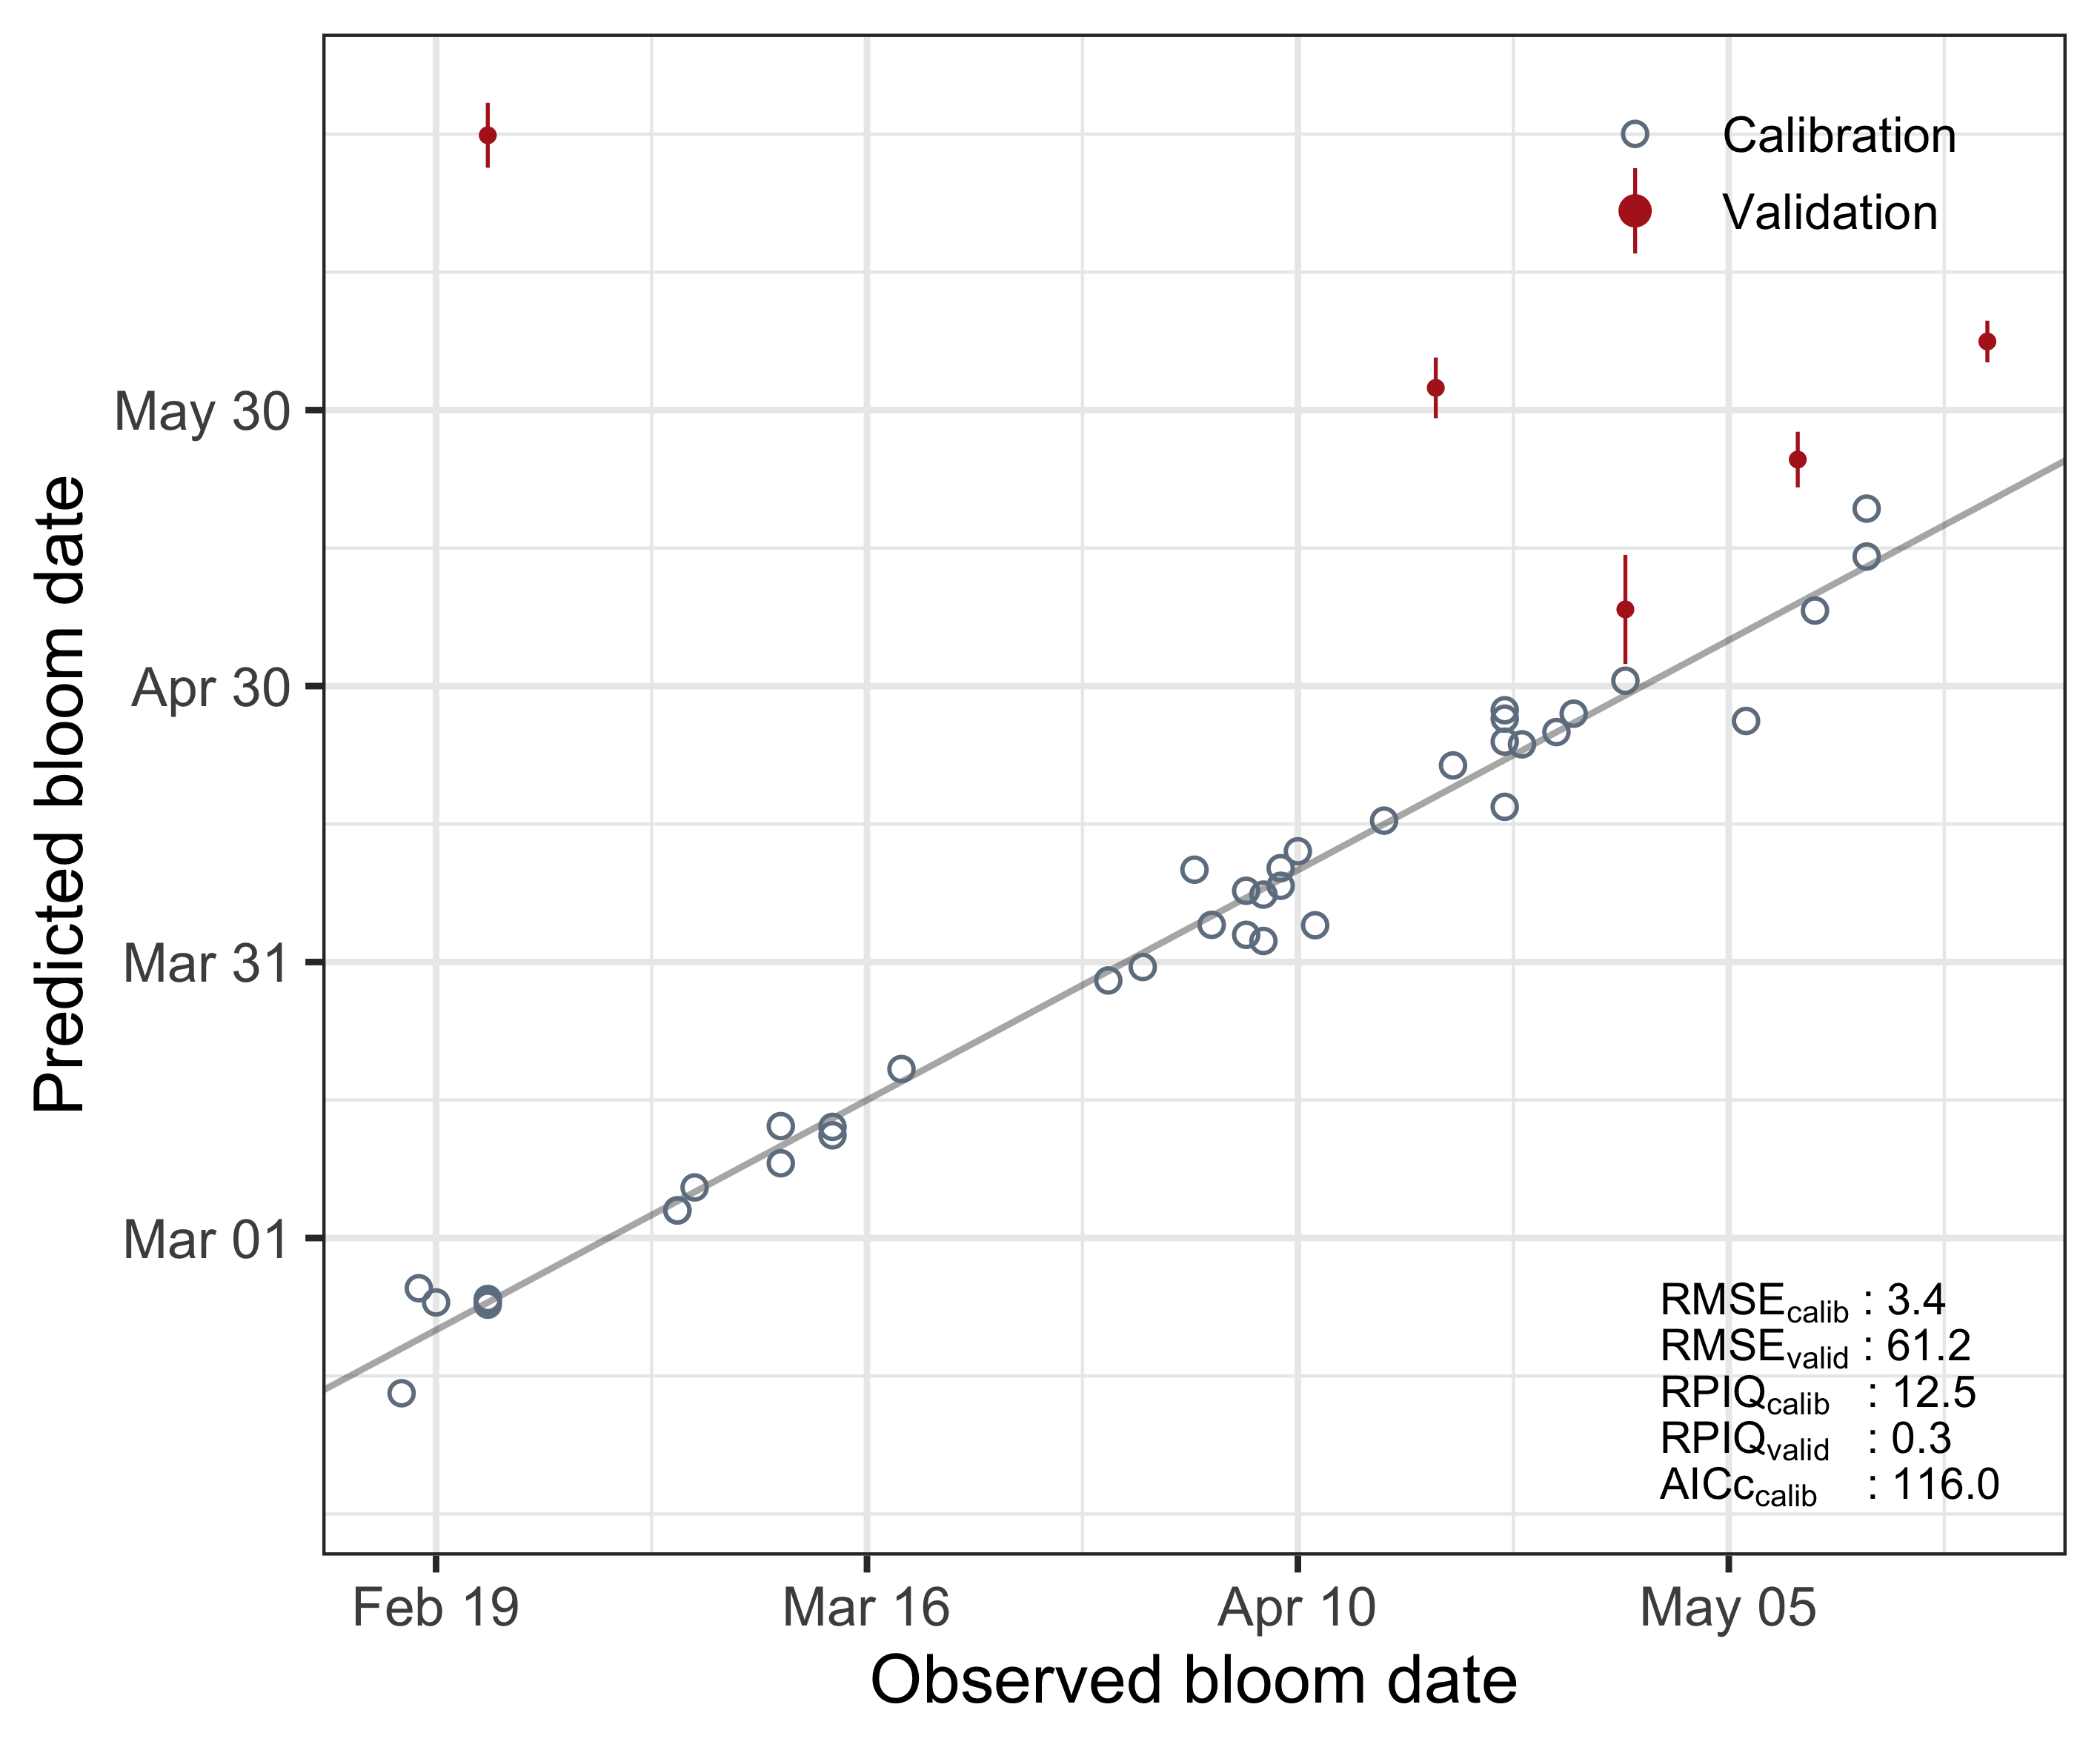
\includegraphics[width=1\linewidth]{figures/final_figures/Figure_S1} 

}

\caption{Validation of the PhenoFlex    extsubscript{excluded} version using the five marginal seasons excluded from the calibration data set. Whereas the open blue circles represent the experimental seasons used for calibration, the filled red circles represent the five marginal seasons used for validating the framework. The vertical lines in the marginal season dots represent the uncertainty estimated by bootstrapping.}\label{fig:fig_s4}
\end{figure}

\newpage

\hypertarget{references}{%
\section*{References}\label{references}}
\addcontentsline{toc}{section}{References}

\hypertarget{refs}{}
\begin{CSLReferences}{1}{0}
\leavevmode\vadjust pre{\hypertarget{ref-Fernandez2021}{}}%
Fernandez, E, P Krefting, A Kunz, H Do, E Fadon, and E Luedeling. 2021.
{``Boosting Statistical Delineation of Chill and Heat Periods in
Temperate Fruit Trees Through {multi-environment} Observations.''}
\emph{Agricultural and Forest Meteorology} 310, 108652.
\url{https://doi.org/10.1016/j.agrformet.2021.108652}.

\leavevmode\vadjust pre{\hypertarget{ref-R-chillR}{}}%
Luedeling, Eike. 2021. \emph{chillR: Statistical Methods for Phenology
Analysis in Temperate Fruit Trees}.

\leavevmode\vadjust pre{\hypertarget{ref-Luedeling2021}{}}%
Luedeling, Eike, Katja Schiffers, Till Fohrmann, and Carsten Urbach.
2021. {``PhenoFlex - an Integrated Model to Predict Spring Phenology in
Temperate Fruit Trees.''} \emph{Agricultural and Forest Meteorology}
307: 108491. \url{https://doi.org/10.1016/j.agrformet.2021.108491}.

\end{CSLReferences}

\end{document}
